\chapter{Results}
\label{chapter:results}

Figure \ref{fig:initial} shows the resulting probability density distributions for the simulated science data loss across the three frameworks. \\
\begin{figure}[h!]
  \centering
  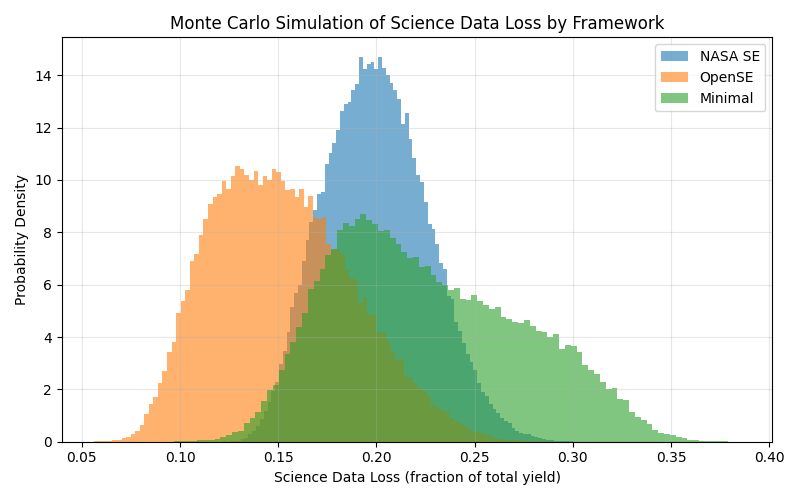
\includegraphics[width=0.9\linewidth]{figures/initial_distribution.png}
  \caption{Initial Scientific Yield Loss Monte Carlo Distribution}
  \label{fig:initial}
\end{figure}

NASA SE displays a narrow, low-loss distribution consistent with highly structured engineering control. OpenSE exhibits a broader spread with a slightly higher mean loss, reflecting its iterative and flexible implementation approach. The Minimal workflow demonstrates the widest spread and highest probability of significant loss, indicative of unmanaged variability and weak lifecycle controls.\\

The summary statistics for all three frameworks are shown in Table \ref{tab:results_summary}. \\
\begin{table}[htbp]
  \centering
  \caption{Summary of Statistics}
  \label{tab:results_summary}
  \begin{tabular}{lccc}
    \toprule
    \textbf{Metric} & \textbf{NASA SE} & \textbf{OpenSE} & \textbf{Minimal} \\
    \midrule
    Mean $L$             & 0.200 & 0.152 & 0.226 \\
    Std.\ $L$            & 0.026 & 0.036 & 0.048 \\
    5th Percentile       & 0.158 & 0.100 & 0.157 \\
    95th Percentile      & 0.245 & 0.216 & 0.312 \\
    $P(L > 10\%)$        & 1.000 & 0.950 & 1.000 \\
    \bottomrule
  \end{tabular}
\end{table}

The probability of exceeding 10\% science data loss, $P(L>0.1)$, was lowest for NASA SE and highest for the Minimal case, with OpenSE positioned in between—suggesting that moderate formalism combined with agility may reduce risk without incurring excessive process overhead.
